\section{Crawling}
\subsection{Document Data}
The dsplearn-admin page was built to allow admins to crawl document data from the Document Server and store into the MySQL database. There are multiple books and text versions in the Document Server. As shown in Figure \ref{fig:dsplearn_admin}, the page displays the date and time of last crawl and allows selection of books and a text version for crawling. 

\begin{figure}[!htbp]
  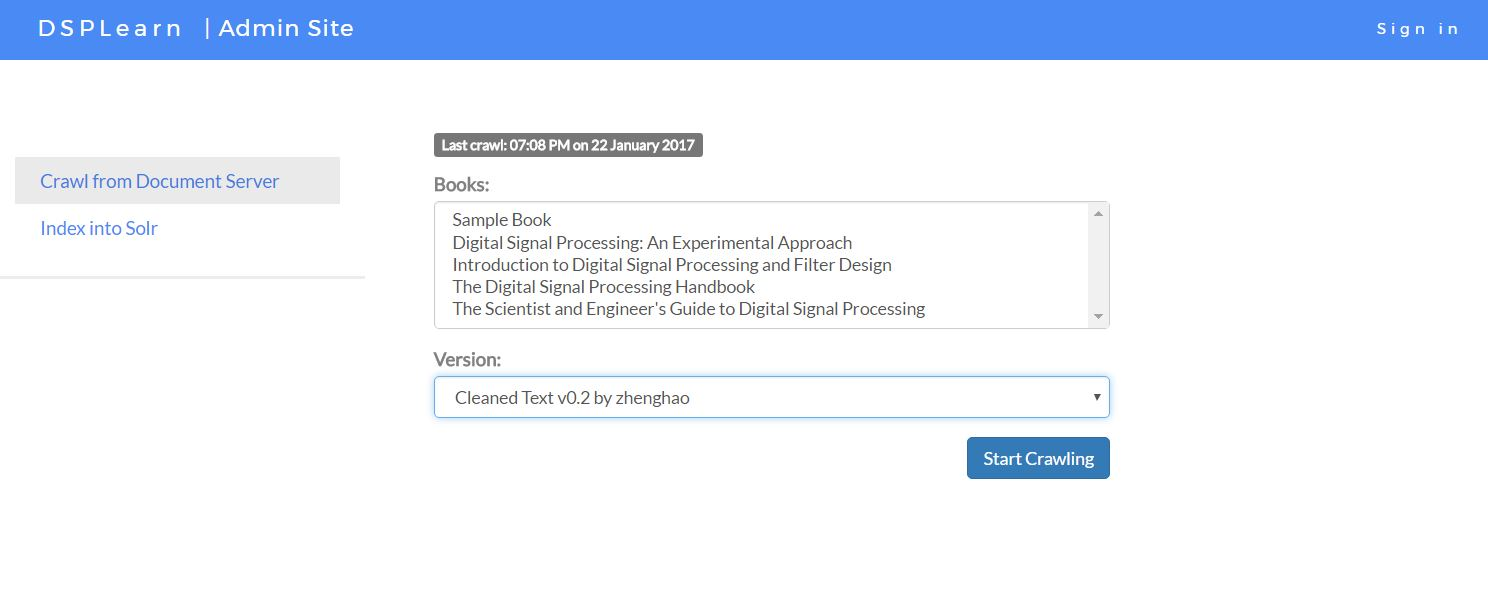
\includegraphics[width=\textwidth]{system_demonstration/demo_dsplearn_admin.jpg}
  \caption{DSPLearn Page for Crawling}
  \label{fig:dsplearn_admin}
\end{figure}

The crawling process is run in the background. Users are kept updated of the crawling status in the web interface, as shown in Figure \ref{fig:sfig:running}.

When some crawling process is running, any other requests for crawling, either from the same user or other users, would be denied, as shown in Figure \ref{fig:sfig:denied}.

When crawling is successfully done, a success message would appear (Figure \ref{fig:sfig:success}) and all crawled document data can be accessed in the MySQL database and the \texttt{Media} folder.

As seen in Figure \ref{fig:media_folder}, all PDF files are organized into two directories \path{books/} and \path{sections/}, with book or section IDs being the file names.

\begin{figure}[!htbp]
\centering
 
  \begin{subfigure}{\textwidth}
  \centering
  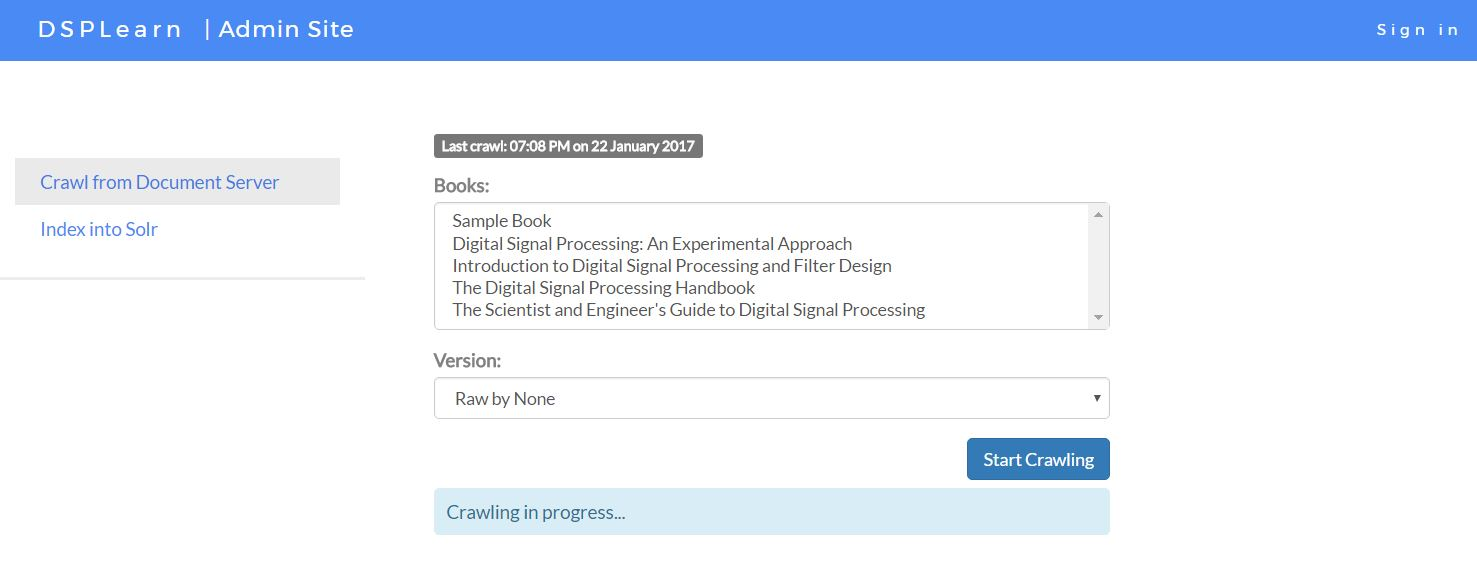
\includegraphics[width=\linewidth]{system_demonstration/demo_crawl_status_running.jpg}
  \caption{In Progress}
  \label{fig:sfig:running}
  \end{subfigure}
  
  \begin{subfigure}{\textwidth}
  \centering
  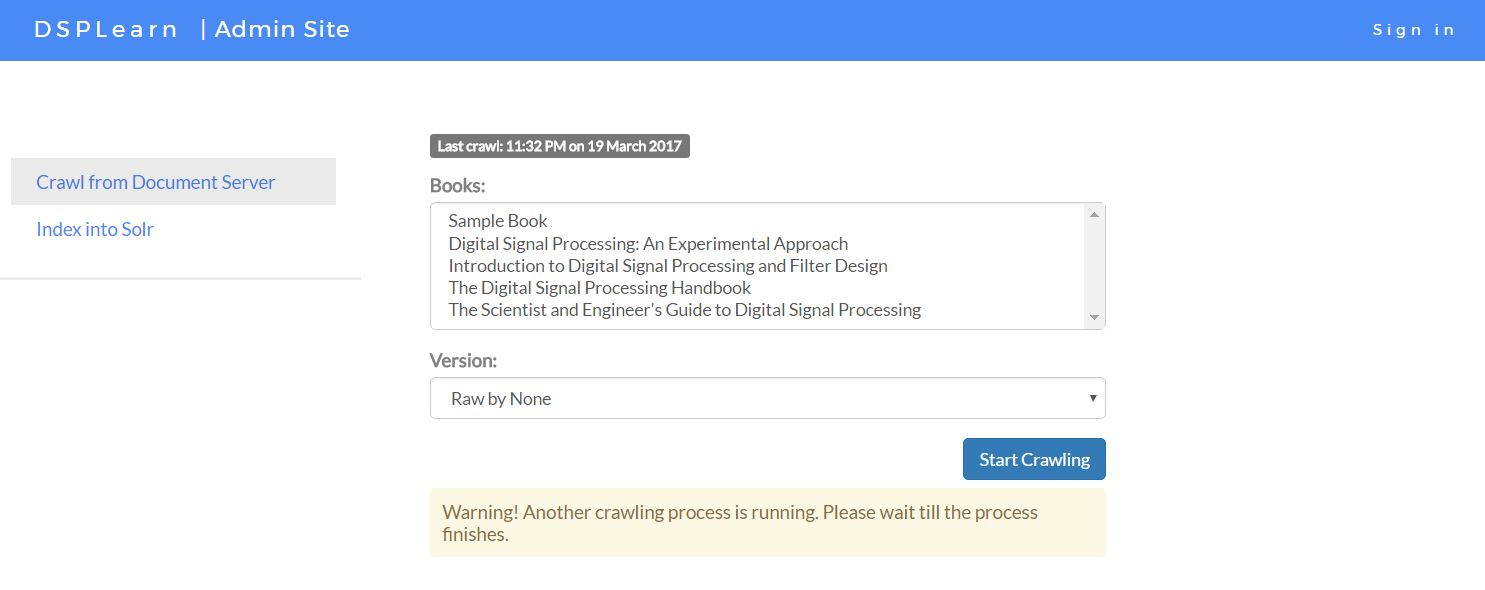
\includegraphics[width=\linewidth]{system_demonstration/demo_crawl_status_warning.jpg}
  \caption{Another Process Running}
  \label{fig:sfig:denied}
  \end{subfigure}
  
  \begin{subfigure}{\textwidth}
  \centering
  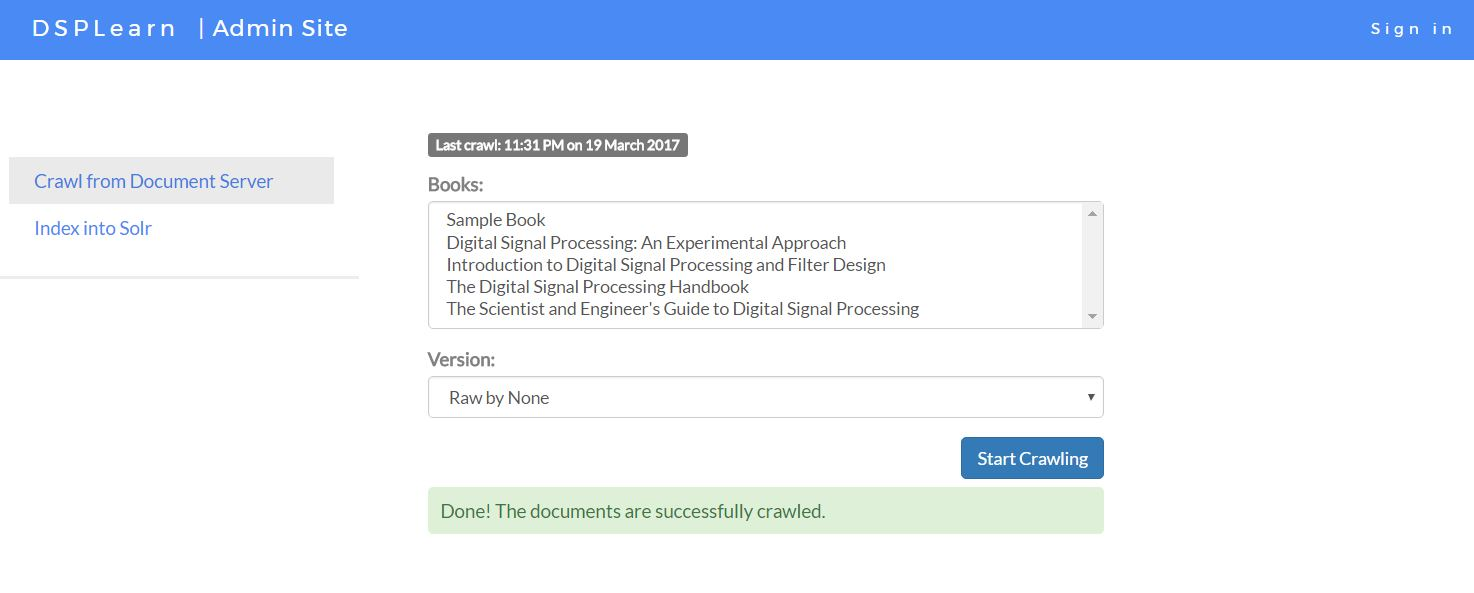
\includegraphics[width=\linewidth]{system_demonstration/demo_crawl_status_success.jpg}
  \caption{Success}
  \label{fig:sfig:success}
  \end{subfigure}
 
\caption{Crawling Status Update}
\label{fig:crawl_status}
\end{figure}

\begin{figure}[!htbp]
  \centering
  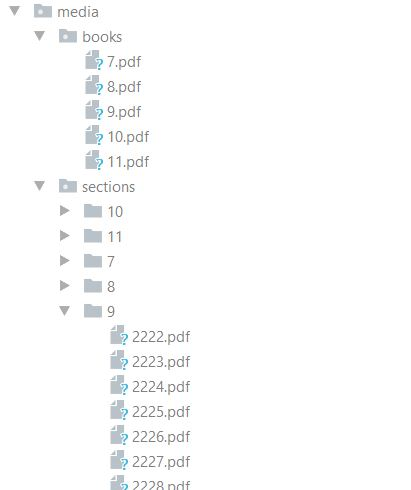
\includegraphics[width=0.6\textwidth]{system_demonstration/demo_media_folder.jpg}
  \caption{\texttt{Media} folder in the Application Server}
  \label{fig:media_folder}
\end{figure}

Figure \ref{fig:django_admin} is the django-admin page. You may access data for all 4 table - \texttt{Books}, \texttt{Concept mappings}, \texttt{Concepts}, and \texttt{Sections} from this page. All entries in the tables \texttt{Books} and \texttt{Sections} are filled during crawling (Figure \ref{fig:django_admin_section_book}).

\begin{figure}[!htbp]
  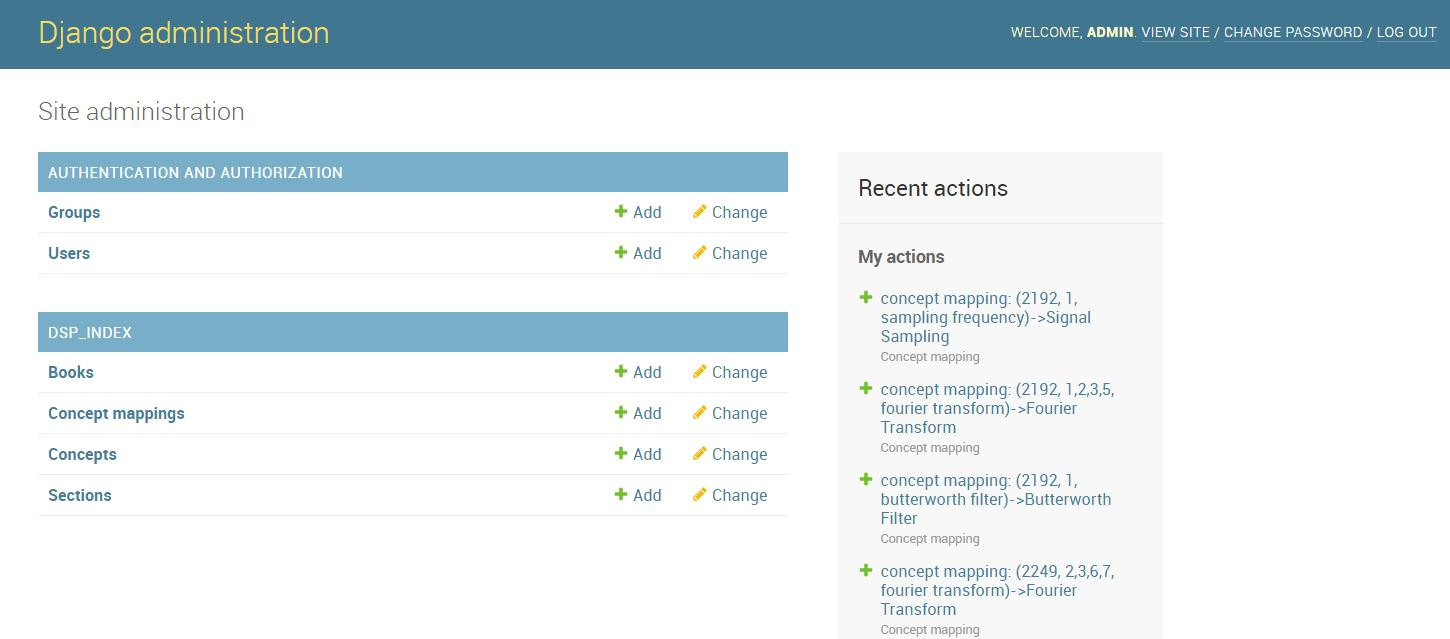
\includegraphics[width=\textwidth]{system_demonstration/demo_django_admin.jpg}
  \caption{Django Admin Page}
  \label{fig:django_admin}
\end{figure}

\begin{figure}[!htbp]
\centering
 
  \begin{subfigure}{\textwidth}
  \centering
  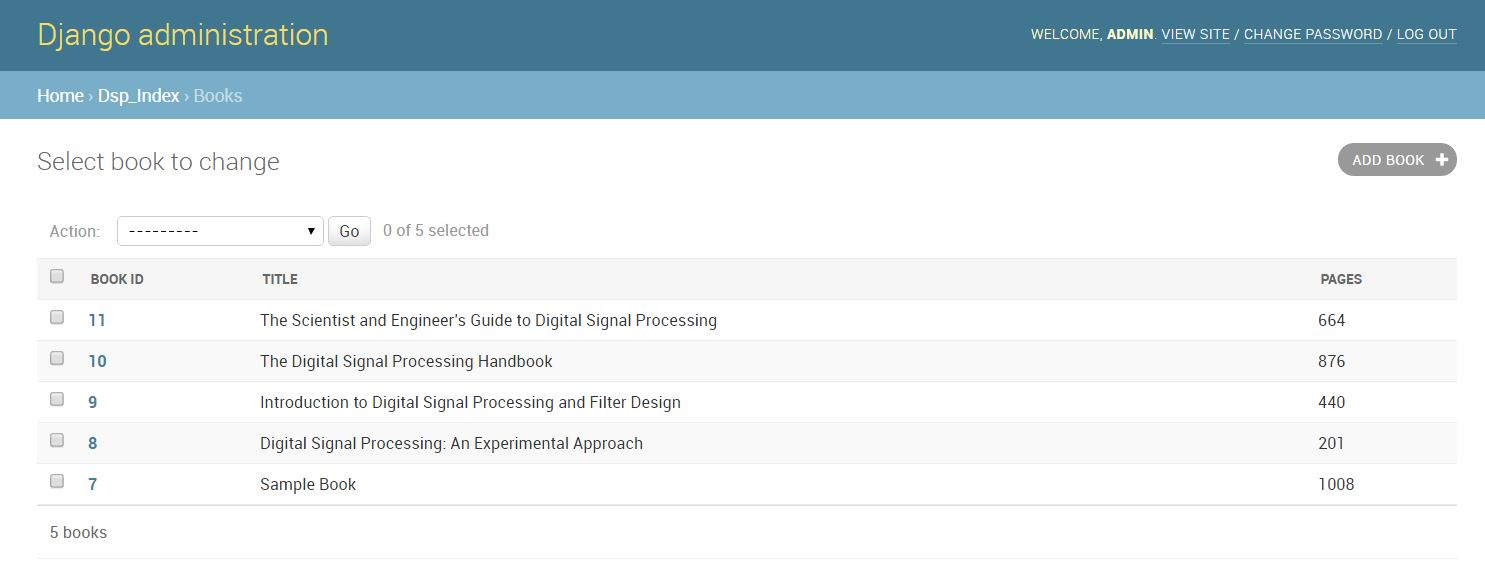
\includegraphics[width=\linewidth]{system_demonstration/demo_admin_books.jpg}
  \caption{\texttt{Books}}
  \label{fig:sfig:admin_books}
  \end{subfigure}
  
  \begin{subfigure}{\textwidth}
  \centering
  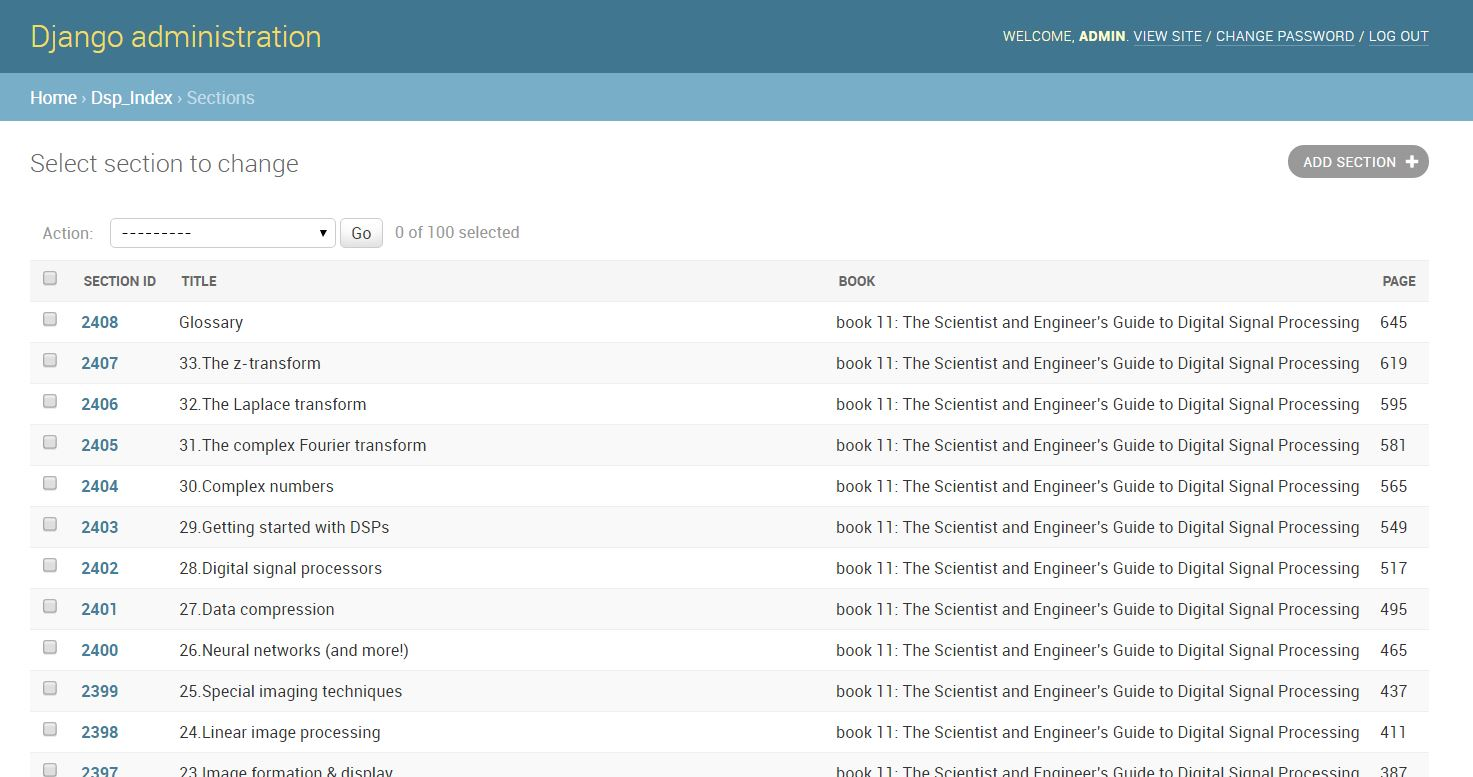
\includegraphics[width=\linewidth]{system_demonstration/demo_admin_sections.jpg}
  \caption{\texttt{Sections}}
  \label{fig:sfig:admin_sections}
  \end{subfigure}
 
\caption{Django Admin Page for \texttt{Sections} and \texttt{Books}}
\label{fig:django_admin_section_book}
\end{figure}

\subsection{Ontology and Term-to-Concept Mappings}
The concept ontology and the term-to-concept mappings are both stored in the MySQL database. Users may add new concept into the existing ontology or drag and drop to modify the ontology (Figure \ref{fig:django_admin_concept_mapping}).

\begin{figure}[!htbp]
\centering
 
  \begin{subfigure}{\textwidth}
  \centering
  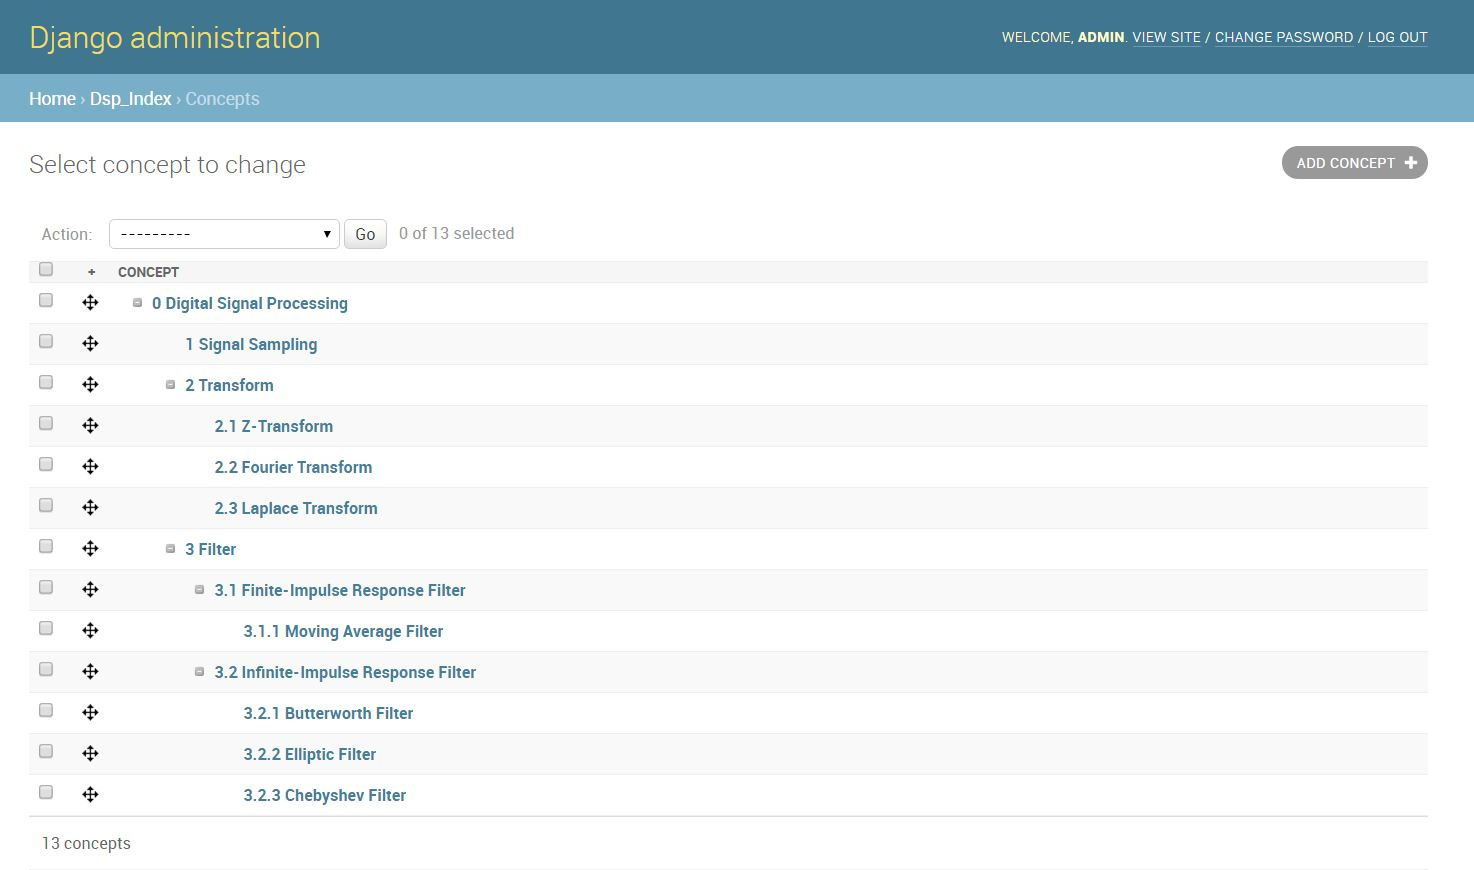
\includegraphics[width=\linewidth]{system_demonstration/demo_admin_concepts.jpg}
  \caption{\texttt{Concepts}}
  \label{fig:sfig:admin_concepts}
  \end{subfigure}
  
  \begin{subfigure}{\textwidth}
  \centering
  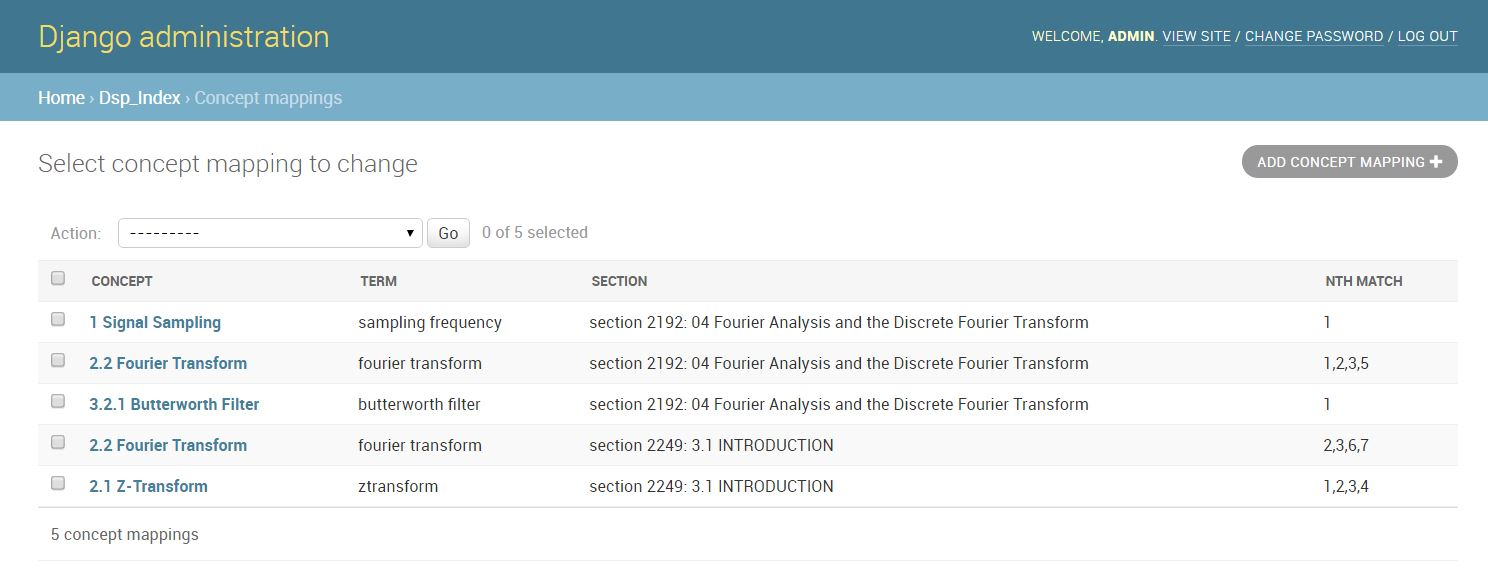
\includegraphics[width=\linewidth]{system_demonstration/demo_admin_concept_mappings.jpg}
  \caption{\texttt{Concept mappings}}
  \label{fig:sfig:admin_mappings}
  \end{subfigure}
 
\caption{Django Admin Page for \texttt{Concepts} and \texttt{Concept Mappings}}
\label{fig:django_admin_concept_mapping}
\end{figure}